%%% LaTeX Template: Article/Thesis/etc. with colored headings and special fonts
%%%
%%% Source: http://www.howtotex.com/

\documentclass[12pt]{article}


\usepackage{apuntes-estilo}
\usepackage{fancyhdr,lastpage}
\usepackage{color,colortbl}
\usepackage{verbatim}

\def\maketitle{

% Titulo 
 \makeatletter
 {\color{bl} \centering \huge \sc \textbf{
 Monitoreo de recursos \\ 
\large \vspace*{-8pt} \color{black} Guía básica de monitoreo de recursos. 
 \vspace*{8pt} }\par}
 \makeatother


% Autor
 \makeatletter
 {\centering \small 
 	Departamento de Ingeniería de Computadoras \\
 	Facultad de Informática - Universidad Nacional del Comahue \\
 	\vspace{20pt} }
 \makeatother

}

% Custom headers and footers
\fancyhf{} % clear all header and footer fields
\fancypagestyle{plain}{\fancyhf{}}
  	\pagestyle{fancy}
 	\lhead{\footnotesize Reconocimiento y monitoreo de recursos - Departamento de Ingeniería de Computadoras}
 	\rhead{\footnotesize \thepage\ }	% ''Page 1 of 2''

\def\ti#1#2{\texttt{#1} & #2 \\ }



\begin{document}

\thispagestyle{empty}
\maketitle
\setlength{\parindent}{0pt}

\section*{Introducción}

Hemos hablado durante un tutorial anterior acerca de reconocimiento de recursos 
físicos, identificar sus características y representación dentro del 
sistema operativo.

Durante este texto nos dedicaremos a observar el consumo de esos recursos 
por parte de los procesos en ejecución. 

Monitorear un recurso significa verificar su estado, es decir si esta 
operando dentro de los parámetros normales. En algunos casos, esto se 
traduce solamente en saber si el recurso está funcionando o no, mientras 
que en otros la definición de operación normal puede ser menos clara. 
Por ejemplo en el caso de un CPU, además de si está presente o no, nos 
interesará saber cuál es su carga de procesos en ejecución. 


\section*{Procesos}

Un proceso es un programa en ejecución. Son digamos, las entidades vivas 
dentro de nuestro sistema. Cada programa que ejecutamos, por ejemplo el 
navegador web, puede disparar la ejecución de uno o mas procesos para 
llevar a cabo su tarea.  A su vez, existen procesos que no son disparados 
por los usuarios, sino que los ejecuta el sistema operativo en sí mismo 
para cumplir sus funciones. Por ejemplo, el proceso \texttt{init}, ó el 
servicio de ssh. 

Los procesos en ejecución necesitan consumir recursos computacionales para 
llevar a cabo su función: CPU, memoria principal (RAM), memoria secundaria, 
transferir datos por red, etc. Algunos procesos necesitarán más tiempo de 
CPU, como puede ser un juego, o un programa de cáluclo; mientras que 
otros, por ejemplo el web browser, necesitarán más memoria principal 
(RAM), etc.

Es la intención de este apunte observar el consumo de recursos por parte de 
los procesos en ejecución. 
 
\subsection*{Estado de los procesos}

El orden en que los procesos reciben la atención de el CPUs, es 
similar a lo que ocurre con las cajas de cobro en un supermercado. 
Imaginemos que cada caja de cobro es un CPU y las personas son los 
procesos. Al igual que en el supermercado, las colas se organizan con 
prioridades, de modo que algunos procesos pueden tener prioridad 
sobre otros a la hora de ser atendidos por el CPU. 

Los procesos no siempre se encuentran en ejecución. 
Como bien sabemos, la cantidad de CPUs disponibles es finita, por ende 
los procesos compiten por 
pequeñas porciones de tiempo de CPU. Momento en el cual, el proceso en 
ejecución tendrá la oportunidad de ejecutar algunas instrucciones de su 
código, hasta en tanto se acabe su porción de tiempo de CPU o bien ocurra 
algún otro evento que evite que el proceso se siga ejecutando (por ejemplo, 
porque está esperando recibir datos de la red). 

Si un proceso necesita abrir un archivo que se encuentra en 
memoria secundaria (disco), habrá una pequeña cantidad de tiempo en la que 
dicho proceso estará esperando por la respuesta del disco, que es muchas 
veces más lenta que la velocidad de procesamiento del CPU. Durante esta
espera, el proceso no está listo para ser ejecutado en CPU, se encuentra 
``durmiendo''. Por lo que, mientras el proceso espera, otros procesos 
pueden aprovechar y ejecutarse en el CPU. 
  
Es así que durante el tiempo de vida de un proceso, este se encontrará en 
diferentes estados. En un sistema GNU/Linux observaremos básicamente 
cinco posibles estados, observables por el adminsitrador de sistemas: 

\begin{itemize}
\item R = Corriendo (running): significa que el proceso se encuentra en 
condiciones de ejecutarse en CPU o bien que está siendo ejecutado.  
\item S = Durmiendo (sleeping): el proceso se encuentra esperando por 
agluna señal o evento, no se encuentra en condiciones de ser ejecutado en 
CPU al momento. 
\item T = Trazado o detenido (traced or stopped): proceso que ha recibido 
la orden de detenerse (por ejemplo a pedido del usuario con el comando 
kill y la señal SIGSTOP). 
\item D = Durmiendo no interrumpible (uninterruptible sleep): se encuentra
esperando por un evento y no puede ser interrumpido. 
\item Z = zombie: proceso que termino y no fue reclamado por su proceso 
padre. 
\end{itemize}

Las trancisiones entre estados siguen el siguiente esquema: 

\begin{center}
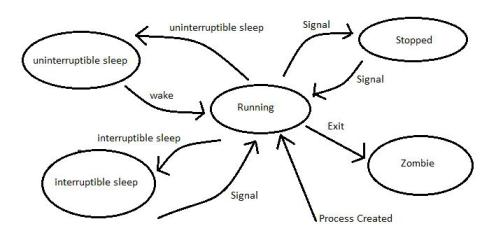
\includegraphics{process-states-s.jpg}
\end{center}
 
Estas transiciones serán en la mayoría de los casos generadas por la misma
funcionalidad del programa, es decir cuando necesita abrir un archivo
estará en estado S, cunado necesita ejecutarse estará en estado R, etc. 
Es decir, el administrador de sistemas, en general no inverviene en las
transiciones de estados. Sin embargo, hay casos en los que esto ocurre. 

\subsection*{Manipulación de procesos}

En el uso cotidiano de un sistema de escritorio, el usuario interviene 
en los estados de los procesos sin darse cuenta. Al pedirle a un programa
que se cierre (por ejemplo apretando la ``X'' en la ventanita), el usuario
le esta pidiendo al proceso que termine y deje de existir. 

El administrador de sistemas en ocasiones deberá manipular el estado de 
los procesos con diferentes fines. Para ello, enviará señales a los 
mismos a través del comando \texttt{kill}. 

El comando \texttt{kill} (matar) tiene una funcionalidad predeterminada, 
equivalente a cerrar un programa desde la interfase gráfica, esto es envía
al proceso la señal SIGTERM (15). El comando 
recibe como argumento una señal y un identificador de proceso (PID) al 
cual enviarle la señal. 

\colorbox{grey}{\parbox[t]{0.95\linewidth}{ \vspace*{0.5cm} { 
{\bf Ejemplo de uso de kill :} \\
{\tt
Sección de la salida del comando \texttt{ps -ef}\\
lechnerm  7324  7320  0 12:40 ?        00:00:00 gnome-pty-helper \\
lechnerm  7325  7320  0 12:40 pts/0    00:00:00 bash\\
lechnerm 10400  7320  0 13:11 pts/2    00:00:00 bash\\
www-data 10725  4250  0 13:12 ?        00:00:00 /usr/sbin/apache2 -k start \\
}
Si, observando la salida anterior, ejecutamos ``\texttt{kill 10725}'', 
estaremos pidiéndole al programa apache2 que termine su ejecución. 
} \vspace*{0.5cm} } } 
	

El comando \texttt{kill} permite, además de su funcionalidad predeterminada,
enviar otras señales que generan otros cambios de estado diferentes al de 
terminar. La lista de señales posibles se pueden listar observando la 
salida del comando \texttt{kill -l}. 
Cada señal tiene un número y un nombre en mayúsculas asociado, cualquiera
de ellos puede utilizarce como argumento del comando \texttt{kill}  

En particular hablaremos de las señales mas frecuentemente utilizadas: 
SIGHUP (1), SIGSTOP (19), SIGCONT(18), SIGTERM (15) y  SIGKILL (9).  


\colorbox{grey}{\parbox[t]{0.95\linewidth}{ \vspace*{0.5cm} { 
{\bf Importante}: cada proceso tiene un usuario dueño (el nombre del
 usuario dueño se observa en la primer columna de la salida de 
\texttt{ps -ef}). El envío de señales a un proceso mediante el 
comando \texttt{kill} sólo pordá realizarlo el dueño o \textbf{root}
} \vspace*{0.5cm} } } 
 


\subsection*{Utilización del CPU}

El CPU es utilizado por cada proceso por períodos cortos de tiempo. Dando 
al usuario, la senación de que todos los procesos corren simultáneamente.
El punto de interés en este caso, es averiguar cuán cargado se encuentra
el o los procesadores de una computadora en un momento particular. El 
primer comando que observaremos es \texttt{uptime}:


\colorbox{grey}{\parbox[t]{0.95\linewidth}{ \vspace*{0.5cm} { 
{\bf Ejemplo de salida de \texttt{uptime}:} \\
{\tt
\# uptime \\
 22:28:41 up 1 day, 22:13, 10 users,  load average: 0,56, 0,65, 0,68
}
} \vspace*{0.5cm} } } 

Este comando muestra la hora actual, el tiempo que hace que el sistema se 
ha iniciado, la cantidad de sesiones iniciadas por usuarios, y la carga 
promedio del sistema en los últimos 1, 5 y 15 minutos. Estos últimos valores
son los de interés en esta sección. 

La carga promedio (load average) representa el número promedio de procesos
que se encuentran ya sea en estado ``ejecutable'' o ``ininterrumpible'' 
(estado ``D'').  Estado ``ejecutable'' puede ser tanto un proceso que se 
encuentra efectivamente ejecutándose en CPU o en cola de ejecución 
(listo para ser ejectudado en CPU).  Se debe tener en cuenta que el valor 
mostrado no se encuentra normalizado por el número de CPUs presentes en 
el sistema, es por esto que un load average de 1 (uno) en un sistema con 
un solo CPU significa que el mismo está cargado todo el tiempo, mientras 
que en un sistema con cuatro CPUs el mismo valor indica que estuvo oscioso
el 75\% del tiempo. 


\begin{center}
 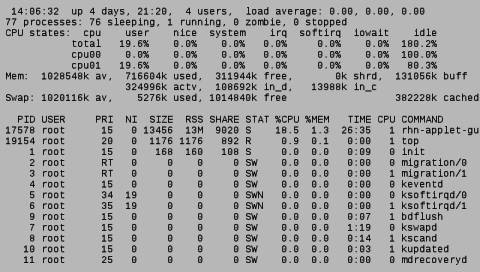
\includegraphics{top.jpg}
\end{center}



\fcolorbox{black}{grey}{
\parbox[t]{1.0 \linewidth}{ \vspace*{0.4cm}
{\bf Lo importante :} Incorporar el hábito de consultar los archivos de log e
identificar la información de interés para el recurso a identificar, o bien la ausencia de la misma.
\vspace*{0.4cm} } }

\colorbox{grey}{\parbox[t]{0.95\linewidth}{ \vspace*{0.5cm} { 
{\bf Ejemplo : Utilizando lscpu }
\\ \\
{\tt \small
\# lscpu \\
Architecture:          i686\\
CPU op-mode(s):        32-bit, 64-bit\\
Byte Order:            Little Endian\\
CPU(s):                2\\
On-line CPU(s) list:   0,1\\
Thread(s) per core:    1\\
Core(s) per socket:    2\\
Socket(s):             1\\
Vendor ID:             AuthenticAMD\\
CPU family:            16\\
Model:                 6\\
Stepping:              3\\
CPU MHz:               800.000\\
BogoMIPS:              5586.01\\
Virtualization:        AMD-V\\
L1d cache:             64K\\
L1i cache:             64K\\
L2 cache:              1024K\\
}
} \vspace*{0.5cm} } } 


\section*{Referencias}

[Intro] Tutuorial Introducción a la Administración de Sistemas GNU/Linux. Materia Introducción
a la Administración de Sistemas. UNCOMA. TUASSL. 

http://www.linuxjournal.com/article/9001


\section*{Licencia}

Este texto fue creado por Miriam Tamara Lechner y se encuentra bajo 
Licencia Creative Commons Atribución-CompartirDerivadasIgual 3.0 Unported

\end{document}
